% 1983 年全国卷（文科）第 9 题：半圆板内接矩形——底边落在直径上、关于过圆心 O 的竖直线对称，矩形上边两顶点在弧上；O 为圆心，R 为半径，图下方以双向箭头标出半径 R（按源卷布局）
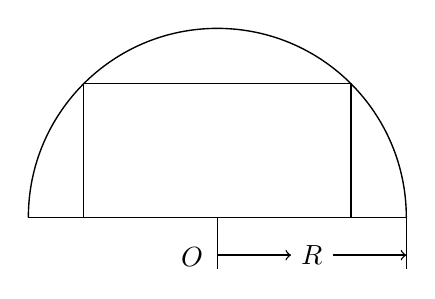
\begin{tikzpicture}[scale=1.2, line width=0.5pt,
  every node/.style={inner sep=1.5pt}]
  % 直径与半圆弧（圆心在原点，半径 2）
  \draw (-2,0) -- (2,0);
  \draw (-2,0) arc (180:0:2);
  % 内接矩形：半底 √2、高 √2（即面积最大时的长宽）
  \draw (-1.4142,0) -- (-1.4142,1.4142) -- (1.4142,1.4142) -- (1.4142,0);
  % 圆心 O 与右端点处的短竖线
  \draw (0,0) -- (0,-0.55);
  \draw (2,0) -- (2,-0.55);
  % 半径 R 的双向箭头（中间留白写 R）
  \draw[->] (0,-0.40) -- (0.78,-0.40);
  \draw[->] (1.22,-0.40) -- (2,-0.40);
  \node at (1,-0.40) {$R$};
  \node[anchor=east] at (-0.10,-0.42) {$O$};
\end{tikzpicture}
